%%%%%%%%%%%%%%%%%%%%%%%%%%%%%%%%%%%%%%%%%%%%%%%%%%%%%%%%%%%%%%%%%%%%%%%%%%%%%%%%
%2345678901234567890123456789012345678901234567890123456789012345678901234567890
%        1         2         3         4         5         6         7         8

\documentclass[letterpaper, 10 pt, conference]{ieeeconf}  % Comment this line out if you need a4paper


%\documentclass[a4paper, 10pt, conference]{ieeeconf}      % Use this line for a4 paper

\IEEEoverridecommandlockouts                              % This command is only needed if 
% you want to use the \thanks command

\overrideIEEEmargins

% Sorts and compresses references properly
% (poor substitute for natbib, but it's the best we can do with this docclass)
\usepackage{cite}

% Give us pretty subfigures
\usepackage{subfig}

% Good math support
\usepackage{mathtools}
\usepackage{amssymb}
\usepackage{graphicx}
\usepackage{caption}
\usepackage{amsmath}
\DeclareCaptionFont{eightpt}{\fontsize{8pt}{9pt}\selectfont #1}
\captionsetup{font=eightpt}

\graphicspath{{figures/}}


\title{\LARGE \bf
	Learning local behavioral sequences 
	to better infer non-local properties in real multi-robot systems
}    
% Automated synthesis of scalable algorithms for inferring non-local
%properties to assist in multi-robot teaming

\author{Taeyeong Choi, Sehyeok Kang, and Theodore P.~Pavlic % <-this % stops a space
	\thanks{*This work was not supported by any organization}% <-this % stops a space
	\thanks{T.~Choi, S.~Kang, and T. P.~Pavlic are with the School of Computing, Informatics, and Decision Systems Engineering,
		Arizona State University, Tempe, AZ 85281, USA
		{\tt\small \{tchoi4, skang66, tpavlic\}@asu.edu}}%
}

\begin{document}
	
	\maketitle
	\thispagestyle{empty}
	\pagestyle{empty}
	
	
	%%%%%%%%%%%%%%%%%%%%%%%%%%%%%%%%%%%%%%%%%%%%%%%%%%%%%%%%%%%%%%%%%%%%%%%%%%%%%%%%
	\begin{abstract}
		
		We propose a more powerful machine learning approach, as an extension of \cite{CPR17},
		to tackle the Remote Teammate
		Localization (RTL) problem where a robot member in a multi-robot team is to predict positions
		of all other teammates only using the observations on its nearest neighbor without any
		communication between robots.
		%        In the previous work, we followed a realistic configuration
		%        in which each robot had a limited sensor radius
		%        As each robot had a relatively simple motion rule with dependency on its nearest neighbors,
		In the previous work, we showed feasibility of a scalable method by which
		a predictor robot was trained in a modular 3-robot team but could extend the prediction
		to a larger
		team without additional training, also suggesting an application of such an inference in
		caging mission.         
		In this work, however, we focus mainly on 1) achieving better performance
		to improve the applicability and 2) conducting evaluation in
		more realistic environments. To be specific, we adopt a Long-Short Term Memory (LSTM)
		to learn possible evolution of behaviors in a modular team helping reduce the errors
		from regression outcomes. Furthermore, while the previous work relied only on computer simulations,
		all the experiments here are conducted on a physical two-wheeled robotic platform, \emph{Thymio},
		to demonstrate the performance gain under realistic constraints.
		
	\end{abstract}
	
	
	%%%%%%%%%%%%%%%%%%%%%%%%%%%%%%%%%%%%%%%%%%%%%%%%%%%%%%%%%%%%%%%%%%%%%%%%%%%%%%%%
	
	\section{Introduction}
	\label{sec:intro}
	
	In multi-robot systems including swarms, every robot is usually allowed to observe 
	only a subset of its team members and interact with them to determine the next action 
	according to relatively simple motion rules. 
	Such a property enables the entire system to perform in a distributed manner, and 
	also the behavior of it can be driven easily by a few leader robots to 
	eventually achieve the goal \cite{CPR17, DGRSS17, EB16, Stern18}. 
	This implies that if a robot has an ability to reognize useful property, e.g.) formation, 
	of the whole team in real time using its local sensors, 
	it could present adjustive actions accordingly to better promote a collective behavior 
	for the sake of the team.
	
	In \cite{CPR17}, we suggested a machine learning method to solve the 
	RTL problem where a robot, called \emph{Tail} at one end of a line formation of 
	a multi-robot team, is to predict positions of all other teammates only using local
	observations about a single nearby teammate. Since each robot has a limited sensor
	radius and a relatively simple motion rule with dependency 
	on the position of its nearest neighbors, 
	the \emph{Tail} has to be able to learn the regularity 
	of the observed motions of neighbor to finally infer the poses of all other robots.
	We introduced a repetitive prediction scheme to use predictions on 
	nearer teammates to make predictions on farther ones until the prediction 
	reached the \emph{Head} robot at the other end in line formation. 	
	Also, computer simulations showed the feasibility of the method 
	especially with caging scenario in which the \emph{Tail} could recognize a
	caging action of \emph{Head} in early stage and promote a proactive maneuver to 
	better assist in team cooperation. 
	
	RTL problem provides some unique characteristics compared to general localization problems. 
	In RTL, the robot does not execute predictions on its own location but on  
	its teammates using accessible information.
	Moreover, the robot is not allowed to communicate with other members during 
	prediction phase to consider communication-free scenarios, which differs from 
	cooperative localization problem. 
	Hence, RTL usually assumes that robots behave with correlations with their neighbors 
	so that the resulting behaviors contain cues about the state of their neighbors. 	
	In this sense, state observers in networked robotic system could be a more similar 
	configuration to RTL, but RTL more emphasizes 
	scalable applications to variable sizes of robot team as well as a general framework 
	that would impose little constraint on dynamics of the system.
	
	%
	\begin{figure}\centering
		\includegraphics[width=1.\columnwidth]{fig_Concept}
		\caption{Illustration of our proposed pipepline in a snapshot example of 
			$5$~robots at time $t$.
			Each robot has a limited view and a motion rule dependent on its neighbors
			except the \emph{Head} robot leading the team at the front. 
			\emph{Tail} uses recent observations on its neighbor, \emph{Follower 3}, 
			which is denoted as $O(t-1,t)$. A sequence of historical poses, $h$, is 
			also encoded for the model to make a final prediction on the 
			unseen teammates. 
		}
		\label{fig:Concept}
	\end{figure}
	%
	
	Figure~\ref{fig:Concept} illustrates our proposed pipeline in which 
	a deep neural network is to learn to synthesize the observations on its neighbor 
	with knowledge about historical positions of all the teammates. 
	As shown in Fig.~\ref{fig:DL_Pipeline}, a LSTM layer is deployed to encode 
	the historical sequence input, which could learn probable evolution of the 
	team shape over time under physical constraints. 
	The sequence encoding could help filter out impossible solution candidates
	that the model might produce if it only utilized the recent observations on 
	the neighbor, as in \cite{CPR17}, 

	Not only a more powerful model but also a more realistic experiment 
	environment are prepared. Previously, we 
	conducted all demonstrations on computer simulations, but in this work, 
	a physical two-wheeled robotic platform, \emph{Thymio} \cite{Shin14}, is mainly 
	used to set up more realistic environments.
	
%	All codes are available online\footnote{http://www.github.com/ctyeong}, and supplementary videos 
%	are submitted as well. 
		
	This paper is organized as follow. 
	In Section~\ref{sec:related_work}, we explore related literature and the distinction of our work. 
	Section~\ref{sec:problem_description} explains more details about our setting of RTL problem. 
	Then, we introduce our method, \emph{IPY-Net}, in Section~\ref{sec:method}, and 
	Section~\ref{sec:experiments} explains details about experiments performed on real robots, 
	including data collection, hyperparameters used for learning, and the results. 
	Lastly, we summarize our research and discuss future directions 
	in Section~\ref{sec:discussion_and_future_work}.

	%
	\begin{figure}\centering
		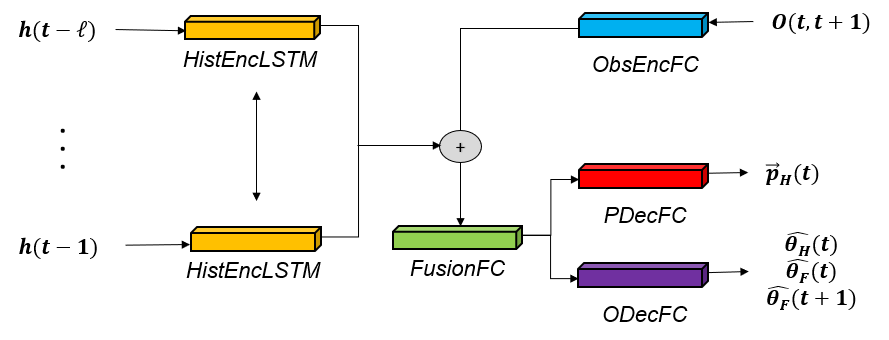
\includegraphics[width=1.\columnwidth]{fig_DL_Pipeline}
		\caption{Structure of our proposed deep neural network. 
			This is an snapshot example when applied to a focused module of
			$3$~robots, called \emph{Tail, Follower, Head} within it, at time $t$. 
			The Encoder-Decoder structure encodes
			1) historical positions and orientations of \emph{Follower} and \emph{Head} 
			until $t-2$ and 2) the observed positions of the \emph{Follower} at $t-1$ and $t$. 
			The decoder part learns to estimate 1) the position of \emph{Head} at $t-1$ and 
			2) orientations of \emph{Follower} at $t-1$ and $t$ and \emph{Head} at $t-1$.   
		}
		\label{fig:DL_Pipeline}
	\end{figure}
	%
	
	
	\section{Related work}
	\label{sec:related_work}
	
	Although the RTL problem is to localize robots, as mentioned in 
	Section~\ref{sec:intro}, it has unique properties compared to conventional 
	localization problems including	cooperative localization or tracking 
	\cite{LSRB16, FSDO10, CX14, DMG15}. 
	It is rather about robot behavior as a container to 
	represent useful team-level state and learning to decode it.
	We discuss related literature below that introduced scenarios to use and decrypt 
	robot behaviors in multi-robot system, followed by a comparison with a work 
	that exploited deep learning to learn dynamics of robot on presentation 
	of force input. 
	Lastly, we explain similarities to our previous work as well as main 
	contributions as an extension.  

	\subsection{Group state recognition}
	\label{sec:group_state_recognition}
	Our approach is basically an attempt to infer positional state of the entire 
	multi-robot team, using only locally obtainable information in the aspect of a robot 
	member. This is because the knowledge about global configuration could 
	help make a better decision for the sake of whole team. In this spirit, 
	the authors in \cite{BG14, BSB16} sampled a subset of robot agents from a swarm to 
	monitor their local interactions and classify the swarm-level behavior. 
	In fact, they implemented relatively simple robots run on a virtual simulator and 
	predefined selections of global behaviors such as \emph{flock} and \emph{torus}. 
	In contrast, our work is to estimate pose of real robots, which would require a more 
	powerful model to regress on any value in a wide range of arena size. 

	\subsection{Behavioral cue interpretation}
	\label{sec:behavioral_cue_interpretation}
	
	One of the main assumptions in RTL is the simple motion rule of each robot which 
	has dependency on the state of its neighbors. This implies that the behavior of 
	neighbors could be a method to encrypt the state change of more remote teammates.
	In \cite{NPCBW12, DCV16}, Novitzky at el. and Das et al. employed a type of
	special action, which appeared like "waggle dance" of honeybees \cite{VonFrisch67}, 
	in robot team so that the behavior could convey a meaning between robots. 
	Our work also encourages a robot to decode behavioral cues, but it occurs without 
	entering an explicit phase of signaling. In other words, the robot has to learn 
	to gain useful information from a sequence of continuous usual interactions. 	
	
	\subsection{Robot dynamics learning}
	\label{sec:robot_dynamics_learning}
	
	Byranvan and Fox in \cite{BF17} proposed a deep learning approach 
	to predict the next visual frame given a current frame and the information 
	of force that would affect one of the shown objects. One of their examples was 
	to understand the dynamics of robotic arms and the relationship with control 
	commands possibly executed. In the RTL problem also, the \emph{Tail} robot may 
	have known 
	a global shape of robot team, and it has to be able to predict the future 
	formation as a new observation on its neighbor is provided, which would encode 
	the information of an unseen force driving the team. Such a similarity inspired 
	the architecture of our neural network model, but they focused on learning 
	motions of rigid objects, while a chain of robots in our work can present 
	much flexibility in team shape. In addition, the force is inferred by 
	movements of the neighbor, which would likely contain noise to some level, while 
	\emph{SE3-Nets} is provided with clear information about the applied force.  
	
	In our previous work \cite{CPR17}, the detailed configurations for RTL 
	problem were first introduced with realistic assumptions. 
	To solve the problem particularly with little robot-to-robot communication, 
	the \emph{Tail} robot is designed to use a repetitive strategy of inference 
	with which the predictions on a closer robot are used as input to 
	prediction for more distant team members. Such an approach enables to scale 
	up the estimation capability without further training even though more robots are 
	added. Albeit we use the same prediction scheme with repetition, here we focus 
	more on developing a more powerful regressor to broaden applicability and 
	also on performing realistic evaluations in a multi-robot system realized on 
	an off-the-shelf robotic platform. 
	
	
	\section{RTL Problem} 
	\label{sec:rtl_problem}
	
	Basically, we follow the problem description for the RTL
	first introduced in \cite{CPR17}. A robot team moves in a line formation 
	in which each robot has two adjacent neighbors except for the ones at the ends, 
	each of which has only one neighbor. 
	The robot on one end is called \emph{Head}, which is the only robot that 
	drives the team toward a destination predetermined in an independent manner.
	The robot on the opposite end is named \emph{Tail}, and all other robots 
	in-between are \emph{Follower}~$i$ where $i \in \{1, 2, ..., n-2\}$ starting
	from the robot closest to the \emph{Tail}.
	Every robot has the same capability of sensor and motion under the same 
	kinematic constraints, although they may take different actions according to 
	motion rules depending on their roles, as formulated in \cite{CPR17}. This catalyzes the
	 \emph{Follower} robots and the \emph{Tail} to behave based on the current positions of their close neighbors. For simplicity, we assume that every robot 
	 has an ability to accelerate fast enough to always keep the neighbors within their 
	 sensory range.
%	As will be explained in 
%	Section~\ref{sec:experiments}, we utilize the computational, sensory capacity of a central 
%	computer in experiments. Therefore, technically the global positions are used to calculate the next 
%	spatial destination of each robot, and then the formula in [] helps generate an actual motion 
%	command to operate two wheels to change its pose according to nonholonomic kinematics. 
	
	The RTL is to localize all the teammates from the view of 
	\emph{Tail} only using locally visible information, which is the position of 
	\emph{Follower}~$1$ at every time step. We assume that until a specific time instant 
	$t$, all the information about positions and orientations of all robots 
	have been shared especially with the \emph{Tail} robot, 
	possibly via global communication,
	but from $t+1$, such information becomes no longer available causing a need of the
	localization technique only utilizing local observations.	
	This may simulate some realistic scenarios where 
	an unexpected technical issue occurs at a time point disabling any robot-to-robot
	data	transfer, or the robot team intentionally stops the information 
	sharing when entering some specific regions either for security or for saving on the
	 communication cost.
	 
	
	\section{Method}
	\label{sec:method}
	
	In this section, we introduce more details about our method. First, 
	we briefly revisit the prediction approach, shown in \cite{CPR17}, 
	to train the model on a small team and to be able to produce predictions 
	even on a larger team without additional training. 
	Then, we present the regressor built for learning not only with observations on 
	the neighbor but also with a sequence of past team formations.


	\subsection{Scalable prediction} 
	\label{sec:scalable_prediction}
	
	We refer to the inference scheme of our previous work \cite{CPR17} in which 
	a regressor is trained in a modular subteam of $3$ robots, and when employed 
	for a larger team, repetitive predictions are performed along with the series
	of $3$-robot modular teams until reaching the prediction step for \emph{Head}. 
	More specifically, given a robot team of size $n$, the \emph{Tail} robot 
	is allowed to gain the position of \emph{Follower 1}, $\vec{p}_{F}$ every 
	single time step. Once 
	
	
	\subsection{Neural network}
	\label{sec:neural_network}
	 
	
	
	\section{Experiments} 
	\label{sec:experiments} 
	
	
	\begin{table}[t]
		\label{table:data_description}
		\centering
		\begin{tabular}{|c|c|c|c|c|}
			\hline
						&  Duration & Num. of Samples & Num. of Instances  \\ \hline
			$3$ robots & $100.6$ minutes & $6,975$ & $465$  \\ \hline
			$5$ robots & $45.0$ minutes  & $8,736$ & $208$  \\ \hline
		\end{tabular}
		\caption{Description of data collected from executions of $3$-robot and $5$-robot teams.}
	\end{table}
	
	
	To demonstrate the effectiveness of our method, we employ a physical robotic platform, 
	\emph{Thymio} \cite{Shin14}, which allows to execute a team of small two-wheeled 
	mobile robots. We use a central computer connected with a overhead camera to simulate
	better proximity 
	sensors, a more powerful computing power, and a GPS system that would easily run on each robot in 
	real scenario. 
	Specifically, the central system is set up to detect the locations of robots in real
	time using off-the-shelf computer vision packages 
	and communicate with a \emph{Raspberry Pi} board \cite{Upton14} on each robot to send
	the next command relying on its neighbors. 
	The command was essentially obtained based on the formulation in \cite{CPR17}, but 
    as the robot was asked to move backward, we just set it not to move for its 
	neighbor behind to catch it up, which helped gain smoother trajectories of the team
	and eventually avoid possible collisions between robots. 
	
	Although the experiment setting involves 
	some external computations and sensors due to limited capability of \emph{Thymio}, 
	most of realistic assumptions still hold from the physical constraints and disturbance
	during execution. For better understanding of readers on the prepared environment, 
	we submit a supplementary video. 
	
	Finally, we collected the pose data from two robot teams, one of $3$~robots and one 
	of $5$~robots, that ran separately in an arena of $2.5 m \times 1.9 m$.  
	The location detection was performed at $4$ frames per second at each of
	which a new command was received by each robot. Also, all pose data was 
	collected at the rate of $2$ frames per second, 
	which was not necessarily synchronized with the command timing. 
	We set the length of history to $5$~seconds ($10$~time steps in data recording) and 
	the time window for prediction to the next $8$~seconds ($16$~time steps).  
	Table~\ref{table:data_description} provides details about the collected data
	where a sample refers to a set of coordinates and orientations in a subteam 
	with which a prediction can be performed, and an instance is set of all available samples for $13$ seconds from the entire team. We clustered recordings so that 
	an instance has at least $7$-second time gap to another ensuring
	the motions between separate instances have little dependency. 
	
	$60$\% data from the $3$-robot team is used to train our model, and another $10\%$
	was set aside for validation. At each epoch of training, a validation followed so that
	the learned weights that achieved the best validation performance were saved. 
	The rest of $20\%$ data and all the data from $5$-robot were used to test the model.
	
	Our model is implemented in \emph{Tensorflow} \emph{Python} library \footnote{https://www.tensorflow.org/} 
	to realize the entire pipeline, and it was trained to minimize 
	loss functions such as Euclidean distance and mean absolute errors 
	for position and orientation estimation, respectively.
	
	We compare our proposed model to two different approaches such as: 
	\begin{itemize}
		\item \emph{$2$X Heuristic}: 
		The prediction on \emph{Head} within a modular subteam is performed by doubling the vector 
		$\vec{p}_{F} - \vec{p}_{T}$.
		
		\item \emph{FC}: 
		Two fully connected layers run in the predictor without historical 
		information, which is based on \cite{CPR17}.  
	
	\end{itemize}	

%	\subsection{Data collection} 
%	\label{sec:data_collection}
	
	
%	\subsection{Results} 
%	\label{sec:results}

	\begin{figure}[t]
	\centering
	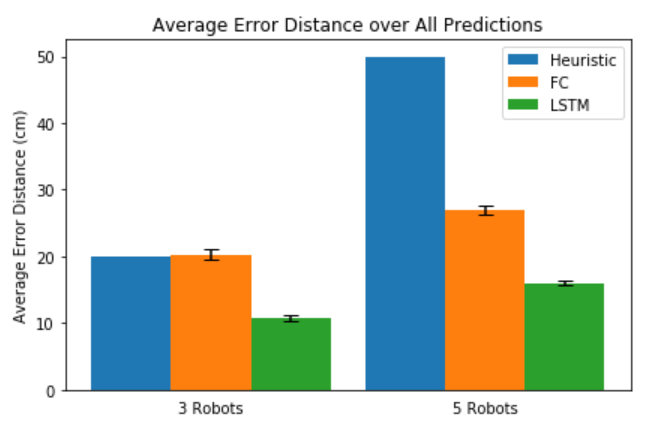
\includegraphics[width=1.\columnwidth]{fig_macro_eval}
	\caption{Average accumulated error of each model in two different sizes of robot team. 
		For each of machine learning methods, the mean performance of $5$~separate training 
		sessions is reported with a error bar to visualize the performance variation. 
	}
	\label{fig:macro_eval}
	\end{figure}


	\begin{figure}[t]
		\centering
		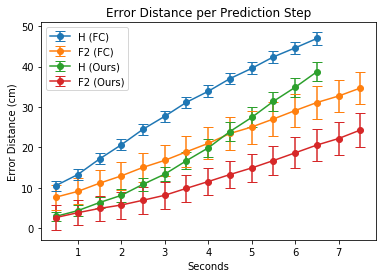
\includegraphics[width=1.\columnwidth]{fig_micro_eval}
		\caption{Average step-wise error for different target robots in $5$-robot team. 
			For each model, all the prediction errors at different time steps are averaged 
			for a specific robot. The error bars represent the standard deviation of 
			$5$~separate models in terms of the performance metric. For the sake of 
			visualization, the error for \emph{Follower~3} is omitted, but note that 
			in any model, the error ranges between the two visualized errors at every step. 
		}
		\label{fig:micro_eval}
	\end{figure}

	
	\subsection{Overall performance}
	\label{sec:overall_performance}
	
	First of all, we evaluate each model in a macroscopic view, as shown in 	
	Fig.~\ref{fig:macro_eval}, where each model is tested with the 
	test data of $3$-robot team and $5$-robot team separately, and in each case, 
	the averaged error for all position predictions is reported. 
	Specifically, in the case of $3$~robots, the average error is calculated only on 
	the prediction for the \emph{Head} robot, while in the $5$-robot case, 
	it involves all predictions for \emph{Follower 2}, \emph{Follower 3}, and \emph{Head}.  
	Moreover, for every model except the \emph{2X Heuristic}, the mean performance of 
	$5$~separate learning sessions is reported with the standard deviation. 
	
	Figure~\ref{fig:macro_eval} displays that the machine learning methods outperform 
	the \emph{2X Heuristic} in any case. In particular, the performance gap between 
	\emph{2X Heuristic} and \emph{FC} becomes much larger in $5$-robot case suggesting that
	during the data collection, we added much randomness to the shape of the robot team.  
	
	Also, our model clearly shows the performance improvement over the \emph{FC} model, since 
	the average error was reduced by $47\%$ and $40\%$ in the $3$-robot and $5$-robot case, 
	respectively. In addition, considering the diameter of a \emph{Thymio} robot is 
	$12$~cm, as only three robots are deployed, the average distance between the prediction 
	and the true position is shorter than the length of the body. This overall result proves 
	the effectiveness of encoding a sequence of historical behaviors as a feature input
	over the model fed only with very recent observation.  

	
	\subsection{Microscopic analysis}
	\label{sec:microscopic_analysis}
	
	In this section, we analyze the performance of the machine learning based models 
	in more fine-grained perspective. For each model, Fig.~\ref{fig:micro_eval} visualizes the 
	step-wise error for different target robots (\emph{Follower 2} and \emph{Head}) 
	in $5$-robot case, which is calculated by averaging the errors of each step across instances. 
	Such a way of evaluation can offer us a crucial insight to understand an approximate time frame 
	within which a level of average error could be ensured for a specific robot. During this 
	evaluation, we also had $5$~separate training sessions to gain the mean and the variability 
	of the performance. 
	
	Figure~\ref{fig:micro_eval} shows that for any target robot, the error increases over time due to the 
	design of the repetitive prediction method where previous errors would negatively 
	impact the prediction power for the following steps. In a similar sense, each model 
	brings about larger error on the \emph{Head} prediction than on the \emph{Follower 2}. 
	
	At every time step, our approach causes less error than the \emph{FC} model for any robot, and  
    the visualized error bars confirm that the performance gap is significant in any case.  
    Especially, for first $4$ seconds, the prediction on \emph{Head} from our model appears 
    more accurate than the prediction on \emph{Follower~2} from the \emph{FC} implying that 
    until then, lower errors is produced on \emph{Follower~3} as well. 
    
    \subsubsection{Limitation} 
	\label{sec:limitation}
	
	Figure~\ref{fig:micro_eval} shows that using our regressor, we could trust the inference 
	outcome until before first $3$~seconds and $4.5$~seconds depending on which robot to target between 
	\emph{Head} and \emph{Follower~2}, since the body of a \emph{Thymio} robot is around 
	$12$~cm. This actually relies on the acceptable degree of error and the diameter of 
	robotic platform used in the problem to tackle. Still, our result demonstrates the potential 
	of effectively alleviating prediction error by adopting a well-designed model, and also, 
	the relatively short time period of guaranteed localization may be sufficient to 
	save on the communication bandwidth within the robot team. 
	
	Also, the error distance when our model performs for \emph{Head} increases relatively slow 
	initially but after some point, the increase rate gradually becomes higher. This is contrast to the 
	case of \emph{FC}, which leads to a constant increase at each time step.  
	This may be because as the historical features are extracted more from previous predictions 
	instead of the truths, it could cause a more accumulated error in prediction outcome than 
	using previous predictions only as observation input as in \emph{FC}.
	
	\begin{figure*}[t]
		\centering
		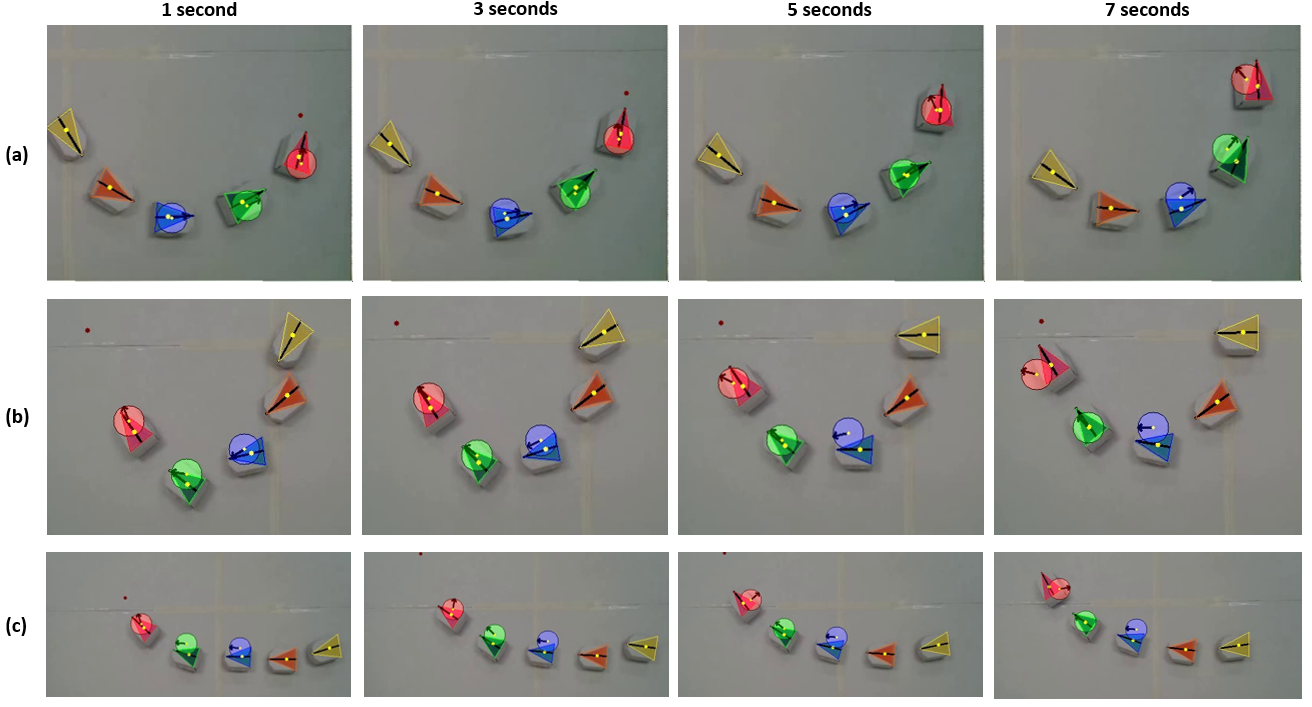
\includegraphics[width=2.\columnwidth]{fig_preds}
		\caption{Sample video frames with prediction results of our proposed model 
			for three different instances of $5$~robot team.
			Each row presents four frames of an instance for first $4$~seconds.   
			The yellow robot is \emph{Tail}, the pink is \emph{Head}, and
			in-between are \emph{Follower} robots. 
			The colored circles are predicted position outputs, in each 
			of which a black arrow is drawn to indicate the predicted orientation as well. 
			The colored triangles with a black line through the center are the 
			results of localization detection used in data collection stage. 
			A small red dot on the arena in each frame is the random destination the 
			\emph{Head} is moving toward, which is resampled at intervals. 
		}
		\label{fig:preds}
	\end{figure*}

	
	\subsection{Qualitative results} 
	\label{sec:qualitative_results} 

	Figure~\ref{fig:preds} displays three different instances of $5$-robot team
	in which both the true positions of all robots and the predictions on them are represented. 
	In overall, the predictions
	until $4$~seconds are shown to be reliable, although there are some errors while the
	group of robots is turning with a high angle and the \emph{Head} changes its destination. 
	An observation is that the predictions tend to be located more inward the curve the team is moving on. 
	Yet, even when the prediction for a nearer robot is away from the truth, the prediction 
	for a farther robot appears correctly in some cases. 
	Such a correction occurs probably because even if an observation input from a nearer robot was 
	actually inaccurate, the past positions in input could alleviate the impact of it and still 
	help generate a decent estimation result.


	\section{Discussion \& Future work}
	\label{sec:discussion_and_future_work}
	
	We have proposed a new design of regression model that can take into consideration 
	the historical behavioral sequences to solve the RTL problem on a real robotic platform. 
	Following the fundamental of scalable localization algorithm introduced in \cite{CPR17}, 
	our approach enables a robot at one end of string of robots to make repetitive predictions 
	on poses of unseen teammates by taking prediction outcomes for nearer robots as input to 
	prediction for farther ones.
	
	We utilized a physical robotic system, \emph{Thymio}, to collect datasets from 
	$3$-robot and $5$-robot teams. Through empirical experiments, we explained that in overall,
	the proposed machine learning model offers more accurate estimation than other baselines.
	In addition, our analysis on timestep-wise errors helped 
	explore the benefits from encoding historical behavior sequences as well as a
	drawback of it. Lastly, we visualized prediction outcomes from a set of samples to 
	illustrate specific cases where the features from past behaviors could also reduce the 
	estimation error passed from previous predictions for nearer robots. 
	
	In the future work, we could more deeply investigate the factors in model accuracy such as 
	the length of history or types of team behavior that might favor the prediction scheme. 
	Also, since the LSTM layer is exposed 
	to various evolutions of team shape during training, the vector representation of it 
	may be examined to characterize team states and finally detect abnormality of the whole
	system. 
	 
	
{\small
	\bibliographystyle{IEEEtran}
	\bibliography{IEEEabrv, IEEEexample}
}


\end{document}
